%!TEX root = ../thesis.tex

\cleardoublepage
\chapter{Introduction}

\label{cha:introduction}

%%=========================================
\section{Motivation and Problem Description}
\label{sec:motivation}

One of the aims for the fifth generation of mobile networks (5G) and it's successors will be a greater diversification of the classes of service. As the use cases for these networks evolve, there is a greater need for quality of service (QoS) tailored to each use case. For example, in the Industrial Internet of Things (IIoT) the requirements on latency, jitter, and reliability may be extremely stringent. Supporting these kinds of classes of service can be a challenge for mobile network operators (MNOs) and will require novel approaches to familiar problems, such as backhaul.

As there are more heterogeneous edge deployments and more campus networks, backhaul becomes more challenging, since many sites may not have access to optical fibre, and may be forced into using other solutions such as satellite links, mmWave backhaul, or pre-existing on-site ISP connections. Providing the kind of deterministic quality of service that these sites may require can be a very difficult challenge.

Network operators may choose to utilize more than one backhaul connection at the same time, in order to increase the available bandwidth or to utilize the different qualities of the backhaul links. This bears the question whether multipathing could then be used to provide deterministic backhaul by intelligently selecting on which links to forward packets. This approach bears similarity to multihoming as well as to multi-path routing in Wireless Sensor Networks (WSNs), and can take inspiration from the existing body of research in these fields, which has demonstrated that QoS can be improved by using multiple links or paths simultaneously \cite{akella2003measurement, tao2005improving, habib2007improving, goldenberg2004optimizing, huang2008multiconstrained, akella2008performance}.


%\LTXtable{\textwidth}{tab/scenario1_sensor}

%%=========================================
\section{Goal}
\label{sec:goal}

\begin{figure}[h]
    \centering
        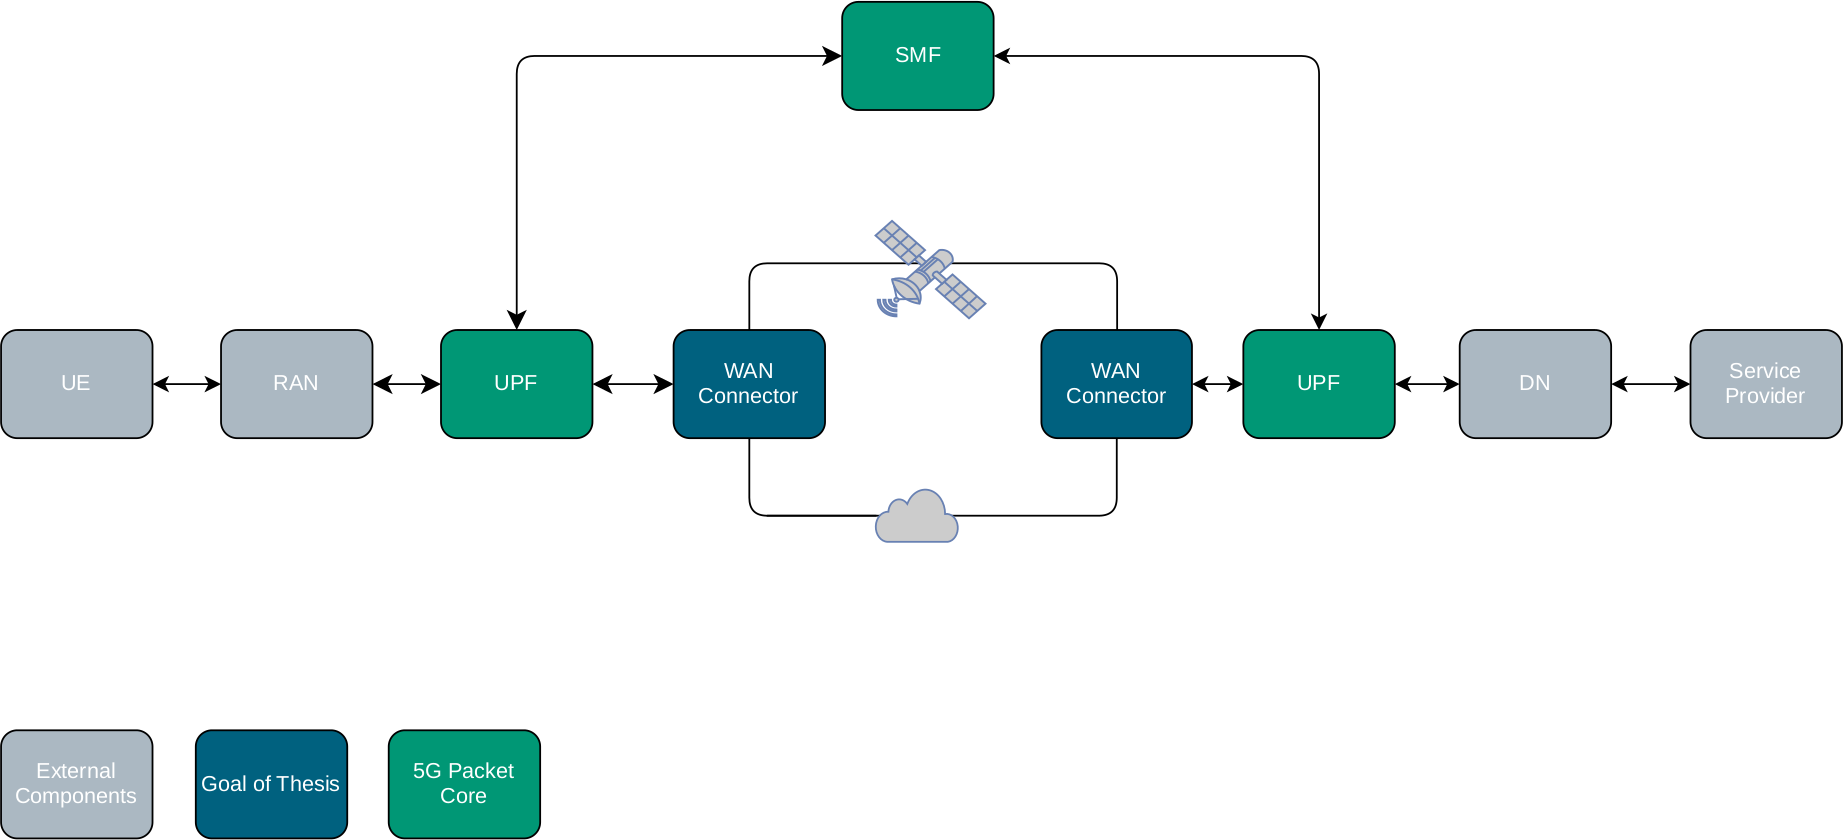
\includegraphics[width=\textwidth]{fig/telco-use-case-2.png}
        \caption{5G Deployment with 2 UPFs}
        \label{fig:telco}
\end{figure}

The goal of this thesis is to design a WAN connector, that can be placed at the ingress and egress point of two or more locations, and utilizes multipathing in order to provide deterministic backhaul between the two sites. The performance of this approach will then be quantitatively analyzed in experiments. Looking at Figure \ref{fig:telco} we can see how this is envisioned to work. WAN connectors are deployed in a geographically distributed 5G campus network, which has more than one egress link, and in the core . Then, using the multiple outgoing links, the traffic is backhauled to the other sites, while respecting it's QoS requirements. This can be especially beneficial for critical applications (e.g. between industrial sites), which are in locations that do not have access to optical fibre for backhaul.

For a 5G deployment the proposed WAN connector could be deployed between multiple User Plane Functions (UPF) and Data Networks (DNs) which also host WAN connectors, in order to provide deterministic backhaul. The architecture for such a deployment is shown in Figure \ref{fig:telco}. Though the on-site UPF is not a strict requirement, it is also feasible to connect the RAN directly to the WAN Connector.

%=======================


\subsubsection{Proposed Solution}

\begin{figure}[h]
    \centering
        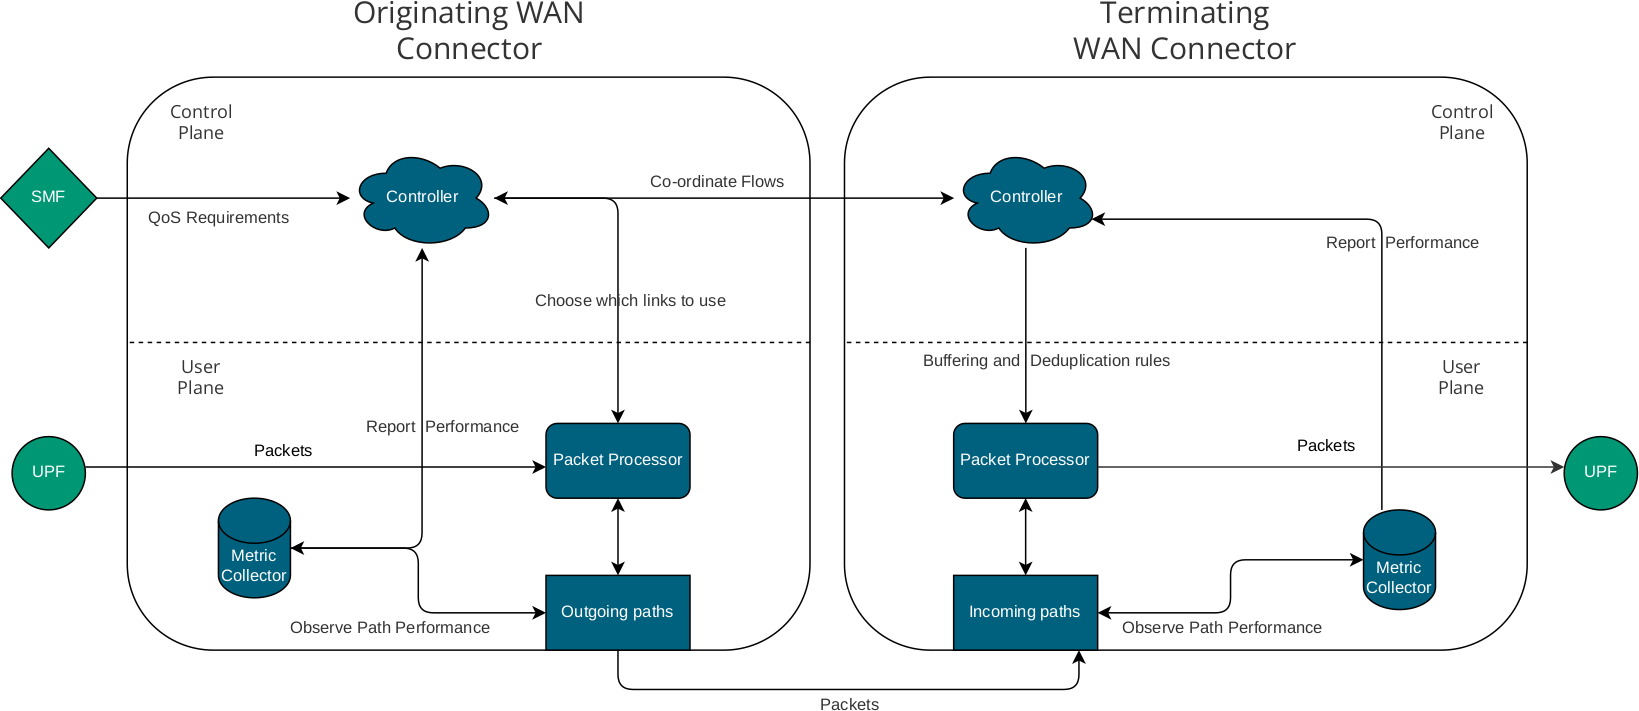
\includegraphics[width=\textwidth]{fig/be-architecture.png}
        \caption{Internal Architecture of the WAN Connector}
        \label{fig:arch}
\end{figure}

The proposed architecture of the WAN connector is shown in Figure \ref{fig:arch}. The connector is split into a control plane, which intelligently chooses which interfaces to forward on, and a data plane, which performs the forwarding, as well as any necessary buffering or en/decoding for forward error correction. The WAN connector also performs different tasks depending on whether it is the origin or termination of a flow. For example, the terminating node may be receiving duplicate packets on the other paths, and it must know to drop these. Or, for example, it may need to wait and accumulate packets before releasing them at a steady rate, in order to reduce jitter (at the cost of higher latency).

Built into this architecture is a module which collects and stores data about the different links, e.g. their latency, reliability, and jitter. When polled, this module reports the performance, and may also try to predict future performance. The link selector uses this information to make its decisions.

\subsection{Evaluating Performance}

In order to evaluate the success of the proposed approach, three scenarios will be set up and investigated. Each setup will consist of two WAN connectors, and some number of emulated links going between them. The first scenario will feature two links emulating regular WAN connections, one link emulating a dedicated line, and one which will emulate a satellite connection. The second scenario will be almost identical to the first but it won't feature the dedicated line, since it is expected that a leased line may be too obvious a choice for any of the traffic with strict QoS requirements. Finally, in order to further investigate these situations where there is an obviously superior candidate, the third scenario will just feature two links: a dedicated line and a WAN link.

\begin{figure}[h]
    \centering
        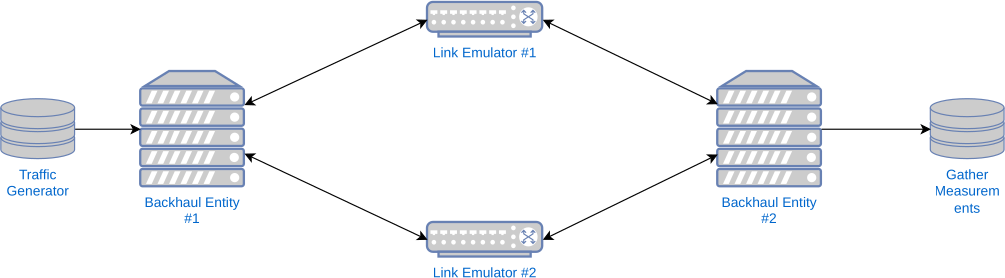
\includegraphics[width=0.66\textwidth]{fig/testbed.png}
        \caption{Testbed Setup}
        \label{fig:testbed}
\end{figure}

In all of these scenarios the same traffic flows will be replayed. This traffic will contain various types of flows, with various QoS requirements. Before a new flow is started, the flow's requirements are sent to the WAN connector and it is either accepted or rejected. During the traffic replay, the delay, jitter, and reliability will be measured.

These measurements will be performed once with the ILP approach proposed earlier and once with a simple round-robin approach for selecting links, and finally compared against an offline approach, where the optimal decision is computed with complete knowledge of the future. This offline approach will serve as the baseline for optimal performance, with which the other two approaches can be compared.

All of these tests can be performed on the same testbed which will be set up as shown in Figure \ref{fig:testbed}. The testbed architecture features a traffic generator, two WAN connectors, with a link emulator between them, and a measurement module to analyze performance. In practice the traffic generator and the test bench will be co-located on the same machine.

%%=========================================



The first phase of the experimental work will consist of setting up the testbed. This means installing the measurement modules as well as the link emulators. The next phase will require the implementation of the WAN connector, as designed. The WAN connector will require a module for collecting per-metric links, as well as the implementation of an algorithm to select the best link or links for a given flow. In the course of designing and preparing the WAN connector there may be room for adjusting the initial plan based on what we experience during development. Next, the connector must be tested. During this phase traffic replays will be played over the testbed and evaluated. Thereafter the round robin approach and the "god routing" approach will also be evaluated. These two approaches will serve for comparison with the performance of the WAN connector. Finally, this data must be analyzed, and the thesis can reach its conclusions, with 1 or 2 weeks buffer room for final revisions.


%%% include all citations

% start zotero

%\nocite{kundel_user_2022}
%\nocite{goldenberg_optimizing_nodate}
%\nocite{lange_performance_2015}
%\nocite{tarique_survey_2009}
%\nocite{tschoke_time-sensitive_2021}
%\nocite{ganichev_yamr_2010}
%\nocite{habib_improving_2007}
%\nocite{tao2005improving}
%\nocite{fanglu_guo_experiences_2004}
%\nocite{akella_measurement-based_nodate}
%\nocite{noauthor_zotero_nodate}

% end zotero...


% google scholar

%\nocite{tsai2006review}
%\nocite{tao2005improving}
%\nocite{kundel2022user}
%\nocite{goldenberg2004optimizing}
%\nocite{lange2015performance}
%\nocite{tarique2009survey}
%\nocite{tschoke2021time}
%\nocite{ganichev2010yamr}
%\nocite{habib2007improving}
%\nocite{guo2004experiences}
%\nocite{akella2003measurement}
%\nocite{ergencc2021reliability}
%\nocite{tao2004application}
%\nocite{alwan2010multi}
%\nocite{prados2021asynchronous}
%\nocite{zhang2016fundamentals}
%\nocite{chen2020collaborative}
%\nocite{akella2008performance}
%\nocite{andreoli2017mobile}
%\nocite{huang2008multiconstrained}
%\nocite{capela2014multihoming}
%\nocite{sheyibani2012reliable}
%\nocite{nguyen2003path}
%\nocite{tao2004exploring}
%\nocite{bremler2002predicting}
%\nocite{zand2012wireless}
%\nocite{li2016multipath}
%\nocite{finn2019deterministic}

